\documentclass{article}
% Semiconductor Process Flow Template

\usepackage[margin=1cm, top=1.5cm, bottom=1.2cm]{geometry}
\usepackage{fancyhdr}
\usepackage{lastpage}
\usepackage{tabularray}
\UseTblrLibrary{booktabs}
\usepackage{xcolor}
\usepackage{helvet}
\usepackage{siunitx}
\usepackage{amsmath}

\renewcommand{\familydefault}{\sfdefault}

% Custom metadata commands with default values
\newcommand{\processflowtitle}{Semiconductor Fabrication Process}
\newcommand{\revision}{Rev 0.0}
\newcommand{\contactemail}{email@example.com}
\newcommand{\contactname}{Name}
\newcommand{\contactphone}{Phone}
\newcommand{\labmanagergroup}{Group}
\newcommand{\batchname}{Batch}
\newcommand{\datecreation}{YYYY-MM-DD}
\newcommand{\daterevision}{YYYY-MM-DD}

% Footer setup
\pagestyle{fancy}
\fancyhf{}
\renewcommand{\headrulewidth}{0pt}
\fancyfoot[L]{\footnotesize Not confidential}
\fancyfoot[C]{\footnotesize File name: \processflowtitle}
\fancyfoot[R]{\footnotesize Page \thepage\ of \pageref{LastPage}}
\renewcommand{\footrulewidth}{0.4pt}

% Title block command using tabularray
\newcommand{\titleblock}{%
    \centering
    \large
    \begin{tblr}{
        width = \textwidth,
        colspec = {X[1.5,l] X[5,l] X[1.5,l] X[5,l]},
        row{1} = {font=\bfseries},
        row{2} = {abovesep=3pt, belowsep=3pt},
        row{3} = {abovesep=3pt, belowsep=3pt},
        cell{1}{1,3} = {font=\bfseries},
        hlines = {0.5pt, white}, % Hidden lines for alignment
        vlines = {0.5pt, white}, % Hidden lines for alignment
        rowsep = 4pt,
        colsep = 8pt,
    }
        Process flow title: & \processflowtitle & Revision: & \revision \\
        Contact email: & \contactemail & Contact name: & \contactname \\
        Contact phone: & \contactphone &  &  \\
        LabManager group: & \labmanagergroup & Batch name: & \batchname \\
        Date of creation: & \datecreation & Date of revision: & \daterevision \\
    \end{tblr}
    \vspace{1em}
    \hrule height 1pt
    \vspace{2em}
}

% Override default metadata
\renewcommand{\processflowtitle}{Minimal MOS Capacitor Process}
\renewcommand{\revision}{Rev 0.3}
\renewcommand{\contactemail}{jephin@dtu.dk}
\renewcommand{\contactname}{Jeppe Hinrichs}
\renewcommand{\contactphone}{Not applicable}
\renewcommand{\labmanagergroup}{Not applicable}
\renewcommand{\batchname}{TBD}
\renewcommand{\datecreation}{2025-08-15}
\renewcommand{\daterevision}{2025-08-19}

\begin{document}

% First page with title block
\titleblock

% ==== DOCUMENT CONTENT ====
\section*{Process Overview}

Minimal MOS capacitor fabrication flow. \\

\subsection*{Key Specifications}
\begin{itemize}
    \item Gate oxide: \qty{35}{\nano\meter} thermal SiO\textsubscript{2}
    \item Gate electrode: \qty{400}{\nano\meter} n+ polysilicon
    \item Backside contact: \qty{400}{\nano\meter} aluminum
\end{itemize}

\subsection*{Critical Safety}
\begin{itemize}
    \item \textbf{HF handling:} Apron+gloves, face shield, no lone working, no glass beakers!
    \item \textbf{Furnace:} Thermal gloves for >\qty{800}{\degreeCelsius} operations
    \item \textbf{Metal anneal:} confirm Al spiking risk mitigated by Ti barrier, avoid $\ge \qty{450}{\degreeCelsius}$ for Al
\end{itemize}

% === MATERIAL SPECIFICATIONS ===
\section{Starting Material}
\begin{tblr}{
    colspec = {lcc},
    row{1} = {font=\bfseries},
    row{2} = {abovesep=3pt,belowsep=3pt}
}
\toprule
Substrate & Specification & Thickness & Qty \\
\midrule
Silicon & p-type <100>, 6", 1-10 \Omega\cdot cm & \qty{500}{\micro\meter} $\pm$ \qty{20}{\micro\meter} & 5 \\
\bottomrule
\end{tblr}

% === LAYER SPECIFICATIONS ===
\section{Critical Layers}
\begin{tblr}{
    colspec = {lcc},
    row{1} = {font=\bfseries},
    row{2-5} = {abovesep=3pt,belowsep=3pt}
}
\toprule
Layer & Material & Thickness \\
\midrule
Gate oxide & Thermal SiO\textsubscript{2} & \qty{35}{\nano\meter} \\
Gate electrode & n+ Poly-Si & \qty{400}{\nano\meter} \\
Back barrier/adhesion & Ti & \qty{100}{\nano\meter} \\
Back contact & Al & \qty{400}{\nano\meter} \\
\bottomrule
\end{tblr}


% === PROCESS FLOW ===
\section{Core Process Flow}
\begin{tblr}{
    colspec = {cX[3]lX[2]},
    row{1} = {font=\bfseries},
    row{2-11} = {abovesep=3pt,belowsep=3pt}
}
\toprule
Step & Process & Equipment & Process & Comment \\
\midrule
0.1 & (Optional) LOCOS isolation & \textcolor{blue}{See locos\_v1.DOCX} & \textcolor{blue}{Use if isolation is required} \\
1.1 & Pre-oxidation clean (HF-last) & Wet bench & SC1, SC2, HF (1–2\%), immediate furnace load \\
2.1 & Gate SiO\textsubscript{2} growth & Furnace & \qty{1000}{\degreeCelsius}, dry/wet-dry recipe to \qty{35}{\nano\meter} \\
3.1 & Poly-Si deposition (n+ preferred) & LPCVD & \qty{620}{\degreeCelsius}, \qty{2}{\hour}; \textit{specify in-situ PH\textsubscript{3} or undoped} \\
3.2 & (If undoped) Poly doping + anneal & Diffusion/RTA & POCl\textsubscript{3} or P implant; anneal per spec \\
4.1 & Gate patterning & Aligner + Etch & Mask: capacitor; poly etch (e.g.\ HBr/Cl\textsubscript{2} ICP or TMAH) \\
5.0 & Backside oxide strip & Wet bench & Protect frontside; remove backside oxide with BOE/HF until bare Si exposed; leave edge exclusion \\
5.1 & Backside Ti deposition & Sputter & \qty{100}{\nano\meter} \\
5.2 & Backside Al deposition & E-beam/Sputter & \qty{400}{\nano\meter} \\
5.3 & Contact/forming-gas anneal & RTP/Furnace & \qtyrange{400}{450}{\degreeCelsius}, \qtyrange{20}{30}{\minute}, N\textsubscript{2} or 5\% H\textsubscript{2} in N\textsubscript{2} \\
\bottomrule
\end{tblr}

% === TROUBLESHOOTING ===
\section{Critical Checks}
\begin{tblr}{
    colspec = {lX[3]},
    row{1} = {font=\bfseries},
    row{2-7} = {abovesep=3pt,belowsep=3pt}
}
\toprule
Step & QC Verification \\
\midrule
2.1 & Oxide thickness: \qty{35}{\nano\meter} $\pm$ \qty{1}{\nano\meter} \\
3.1/3.2 & Poly n+ sheet resistance: $\le$ 30~\Omega/\square \\
4.1 & Gate CD: $\pm$ $\qty{0.5}{\micro\meter}$ \\
5.0 & Backside oxide fully removed (contact-angle change, test drop, or monitor wafer) \\
5.1 & Backside Ti sheet resistance $\approx$ 0.3~\Omega/\square (\qty{100}{\nano\meter} Ti) \\
5.2 & Backside Al sheet resistance $\approx$ 0.07~\Omega/\square (\qty{400}{\nano\meter} Al) \\
5.3 & Contact anneal; contact resistance to Si governed by Ti/Si interface quality (target < 1~\Omega \cdot contact) \\
\bottomrule
\end{tblr}

% === PROCESS FLOW DIAGRAM ===
\section{Process Flow Diagram}
\begin{figure}[h!]
    \centering
    \usetikzlibrary{shapes.geometric, arrows, positioning, calc}

\tikzset{
    process/.style = {rectangle, rounded corners,
        minimum width=3.8cm, minimum height=0.9cm,
        text centered, draw=black, fill=blue!10, font=\footnotesize},
    optional/.style = {rectangle, rounded corners,
        minimum width=3.8cm, minimum height=0.9cm,
        text centered, draw=black, fill=gray!15, dashed, font=\footnotesize},
    inspection/.style = {rectangle, rounded corners,
        minimum width=3.8cm, minimum height=0.9cm,
        text centered, draw=black, fill=green!10, font=\footnotesize},
    toolprep/.style = {rectangle, rounded corners,
        minimum width=3.8cm, minimum height=0.7cm,
        text centered, draw=black, fill=orange!10, font=\scriptsize},
    arrow/.style = {thick,->,>=stealth}
}
\begin{tikzpicture}[node distance=0.45cm]

% ========== COLUMN 1 ==========
% Dry-Ox Group
\node (step1) [process] {1.1: Pre-oxidation inspect};
\node (step1a) [optional, below=of step1] {1.2: Pre-clean (optional)};
\node (step2) [process, below=of step1a] {1.3: Gate SiO\textsubscript{2} growth};
\node (step2a) [inspection, below=of step2] {1.4: Oxide inspection};

% Poly-Si Group
\node (step3a) [optional, below=of step2a] {2.1: Pre-clean (optional)};
\node (step3) [process, below=of step3a] {2.2: Poly-Si deposition};
\node (step3b) [inspection, below=of step3] {2.3: Poly inspection};

% Anneal Group
\node (step4a) [optional, below=of step3b] {3.1: Pre-clean (optional)};
\node (step4) [process, below=of step4a] {3.2: Poly-Si anneal};

% Etch Gate Poly Group - Part 1
\node (step5) [process, below=of step4] {4.1: Gate litho - Coat};
\node (step6) [process, below=of step5] {4.2: Gate litho - Expose};
\node (step7) [process, below=of step6] {4.3: Gate litho - Develop};
\node (step7a) [inspection, below=of step7] {4.4: Litho inspection};
\node (step8) [toolprep, below=of step7a] {4.5: DRIE tool prep};
\node (step9) [process, below=of step8] {4.6: Gate poly etch};


% Group Labels for Column 1
\node[left=0.1cm of step1, font=\bfseries\small] {1 Dry-Ox};
\node[left=0.1cm of step3a, font=\bfseries\small] {2 Poly-Si};
\node[left=0.1cm of step4a, font=\bfseries\small] {3 Anneal};
\node[left=0.1cm of step5, font=\bfseries\small] {4 Etch Gate Poly};

% ========== COLUMN 2 ==========
% Start Column 2 to the right of Column 1
% Etch Gate Poly Group - Part 2
\node (step9a) [toolprep, right=5.5cm of step1] {4.7: DRIE tool clean};
\node (step10) [inspection, below=of step9a] {4.8: Etch inspection};
\node (step11) [process, below=of step10] {4.9: Resist strip};
\node (step11a) [inspection, below=of step11] {4.10: Final inspection};

% Backside preparation
\node (step12) [process, below=of step11a] {5.1: Backside oxide etch};

% Backside electrode Group
\node (step13) [process, below=of step12] {6.1: Backside litho - Coat};
\node (step14) [process, below=of step13] {6.2: Backside litho - Expose};
\node (step15) [process, below=of step14] {6.3: Backside litho - Develop};
\node (step15a) [inspection, below=of step15] {6.4: Litho inspection};
\node (step16) [process, below=of step15a] {6.5: Ti deposition};
\node (step17) [process, below=of step16] {6.6: Al deposition};
\node (step18) [process, below=of step17] {6.7: Lift-off};
\node (step18a) [inspection, below=of step18] {6.8: Post-lift-off inspect};
\node (step19) [process, below=of step18a] {6.9: Contact anneal};

% Group Labels for Column 2
\node[above=0.1cm of step9a, font=\bfseries\small] {4 Etch Gate Poly};
\node[left=0.1cm of step12, font=\bfseries\small] {5 Backside prep};
\node[left=0.1cm of step13, font=\bfseries\small] {6 Backside electrode};

% ========== ARROWS ==========
% Arrows in Column 1
\draw [arrow] (step1) -- (step1a);
\draw [arrow] (step1a) -- (step2);
\draw [arrow] (step2) -- (step2a);
\draw [arrow] (step2a) -- (step3a);
\draw [arrow] (step3a) -- (step3);
\draw [arrow] (step3) -- (step3b);
\draw [arrow] (step3b) -- (step4a);
\draw [arrow] (step4a) -- (step4);
\draw [arrow] (step4) -- (step5);
\draw [arrow] (step5) -- (step6);
\draw [arrow] (step6) -- (step7);
\draw [arrow] (step7) -- (step7a);
\draw [arrow] (step7a) -- (step8);
\draw [arrow] (step8) -- (step9);
%\draw [arrow] (step9) -- (step9a);

% Arrows in Column 2
\draw [arrow] (step9a) -- (step10);
\draw [arrow] (step10) -- (step11);
\draw [arrow] (step11) -- (step11a);
\draw [arrow] (step11a) -- (step12);
\draw [arrow] (step12) -- (step13);
\draw [arrow] (step13) -- (step14);
\draw [arrow] (step14) -- (step15);
\draw [arrow] (step15) -- (step15a);
\draw [arrow] (step15a) -- (step16);
\draw [arrow] (step16) -- (step17);
\draw [arrow] (step17) -- (step18);
\draw [arrow] (step18) -- (step18a);
\draw [arrow] (step18a) -- (step19);

% ========== CONNECTING ARROWS ==========
% Connect from Column 1 to Column 2 (within Step 4)
\draw [arrow] (step9.east) -- ++(1,0) |- (step9a.west);

\end{tikzpicture}
    \caption{Process flow diagram for MOS capacitor fabrication.}
    \label{fig:moscap_flow}
\end{figure}

% === FIGURES ===
\section{Required Figures}
\begin{longtblr}{
    colspec = {c c X[3]},
    row{1} = {font=\bfseries},
    row{2-Z} = {abovesep=3pt, belowsep=3pt},
    hlines,
    vlines,
}
ID & Step & Description \\

0 & 0.1 &
\begin{minipage}{\linewidth}
    \centering
    \resizebox{!}{3.5cm}{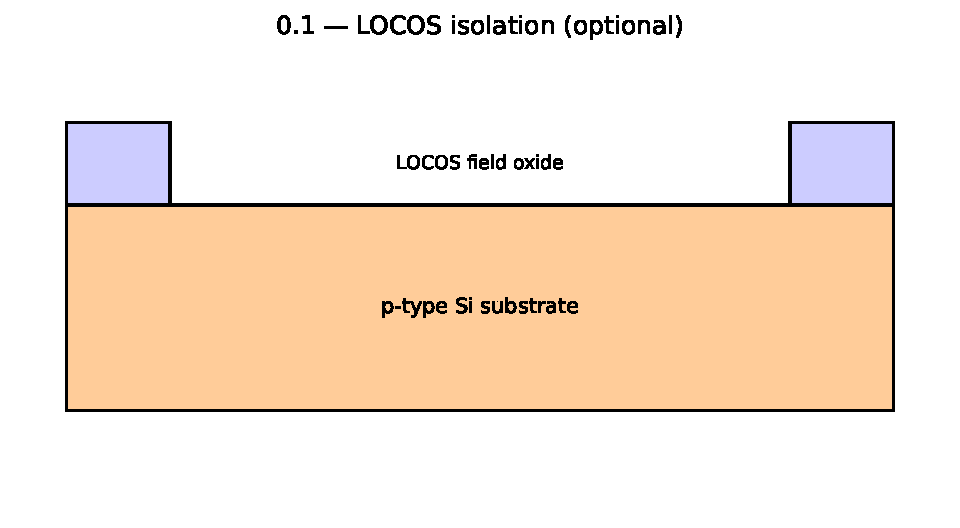
\includegraphics{figures/process_steps/moscap/moscap_step_0-1.pdf}}\\[2pt]
    LOCOS isolation (optional)
\end{minipage} \\

1 & 1.1 &
\begin{minipage}{\linewidth}
    \centering
    \resizebox{!}{3.5cm}{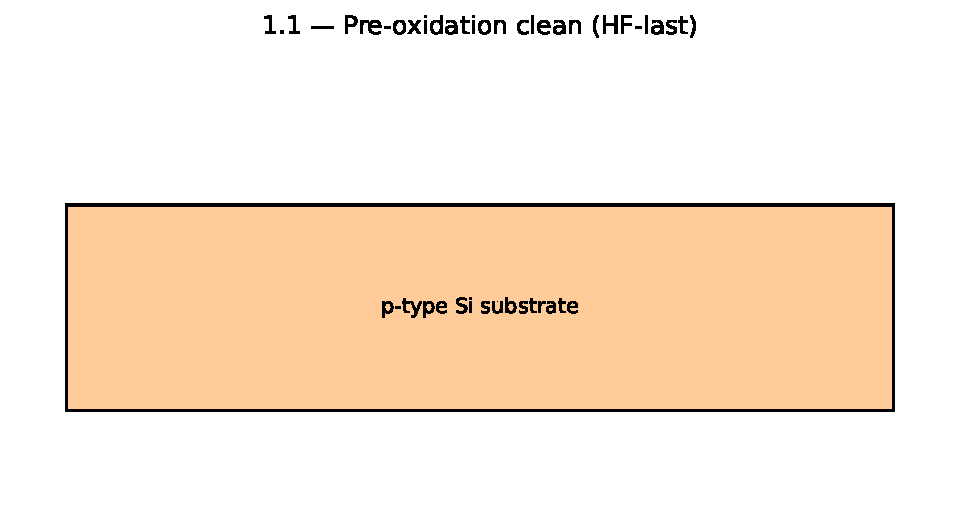
\includegraphics{figures/process_steps/moscap/moscap_step_1-1.pdf}}\\[2pt]
    Pre-oxidation clean (HF-last)
\end{minipage} \\

2 & 2.1 &
\begin{minipage}{\linewidth}
    \centering
    \resizebox{!}{3.5cm}{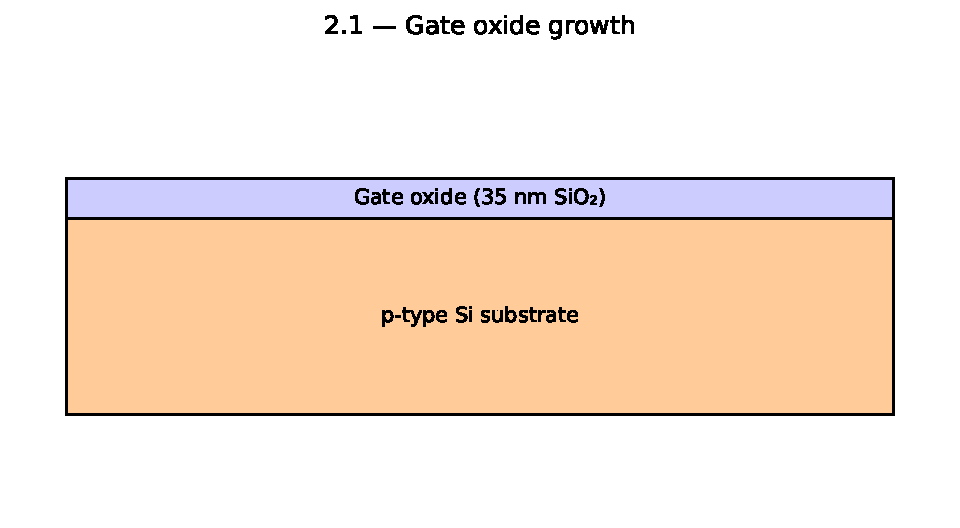
\includegraphics{figures/process_steps/moscap/moscap_step_2-1.pdf}}\\[2pt]
    Gate oxide growth
\end{minipage} \\

3 & 3.1 &
\begin{minipage}{\linewidth}
    \centering
    \resizebox{!}{3.5cm}{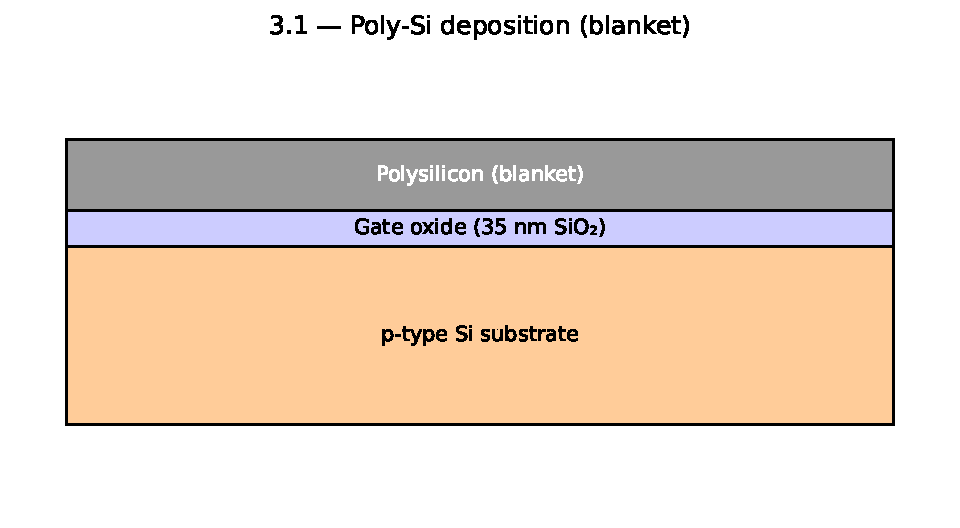
\includegraphics{figures/process_steps/moscap/moscap_step_3-1.pdf}}\\[2pt]
    Poly-Si deposition (blanket)
\end{minipage} \\

4 & 3.2 &
\begin{minipage}{\linewidth}
    \centering
    \resizebox{!}{3.5cm}{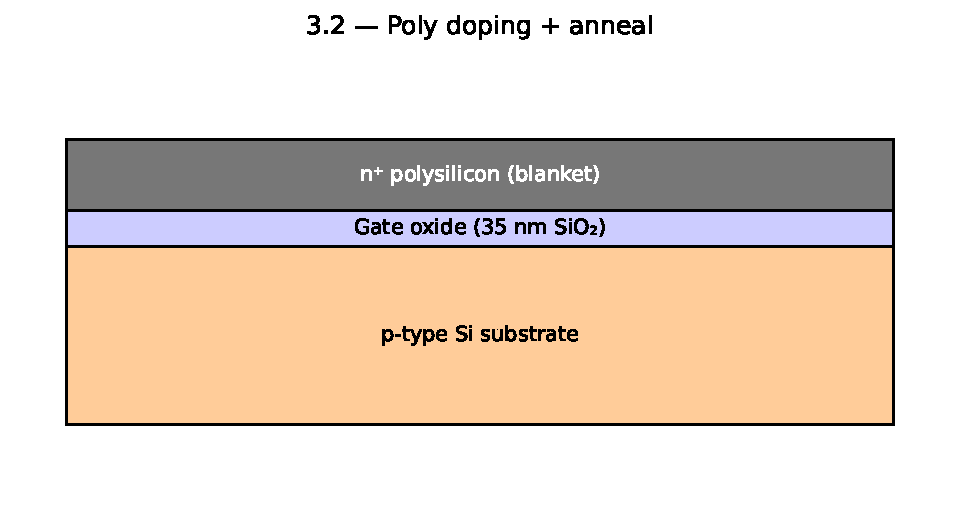
\includegraphics{figures/process_steps/moscap/moscap_step_3-2.pdf}}\\[2pt]
    Poly doping + anneal
\end{minipage} \\

5 & 4.1 &
\begin{minipage}{\linewidth}
    \centering
    \resizebox{!}{3.5cm}{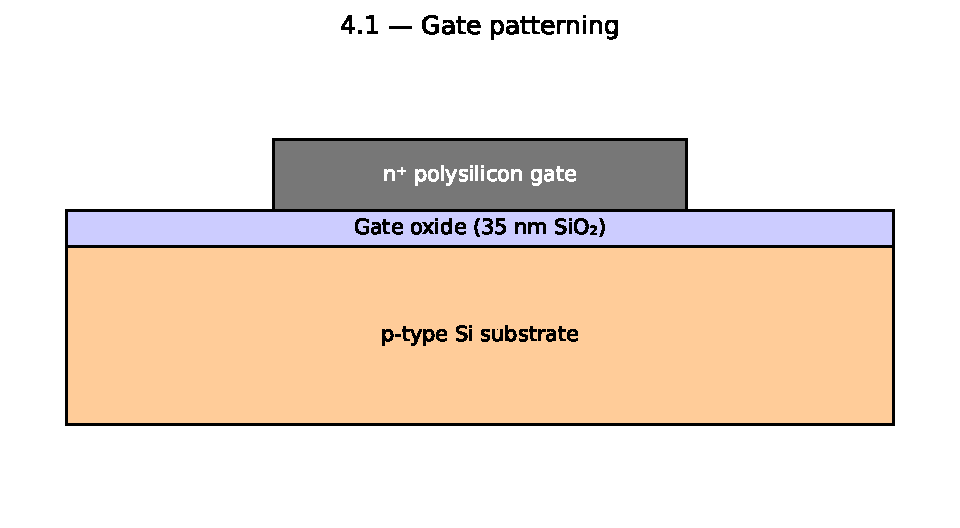
\includegraphics{figures/process_steps/moscap/moscap_step_4-1.pdf}}\\[2pt]
    Gate patterning + top pad
\end{minipage} \\

6 & 5.0 &
\begin{minipage}{\linewidth}
    \centering
    \resizebox{!}{3.5cm}{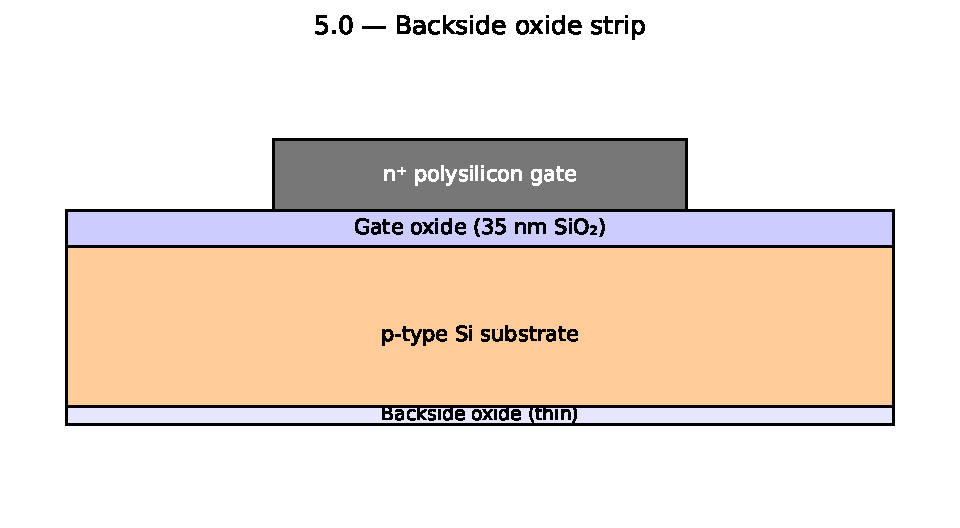
\includegraphics{figures/process_steps/moscap/moscap_step_5-0.pdf}}\\[2pt]
    Backside oxide strip
\end{minipage} \\

7 & 5.1 &
\begin{minipage}{\linewidth}
    \centering
    \resizebox{!}{3.5cm}{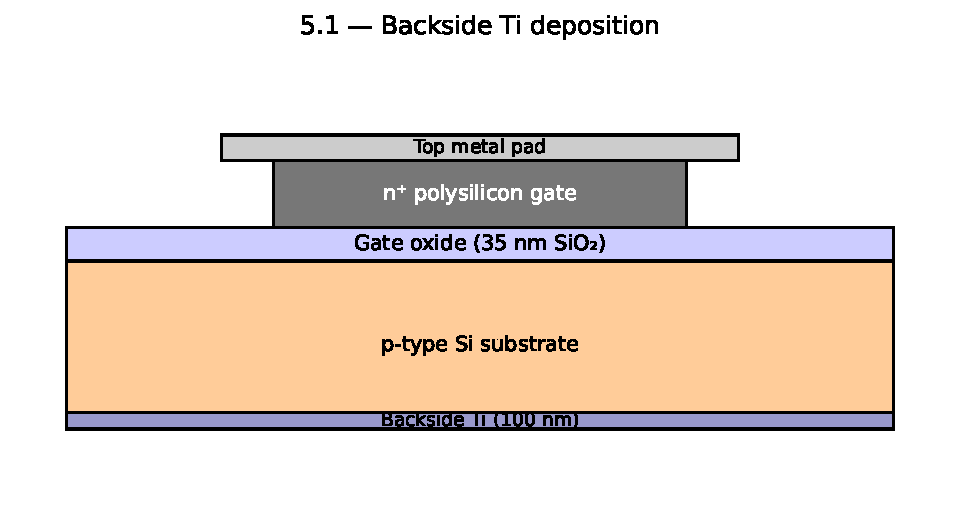
\includegraphics{figures/process_steps/moscap/moscap_step_5-1.pdf}}\\[2pt]
    Backside Ti deposition
\end{minipage} \\

8 & 5.2 &
\begin{minipage}{\linewidth}
    \centering
    \resizebox{!}{3.5cm}{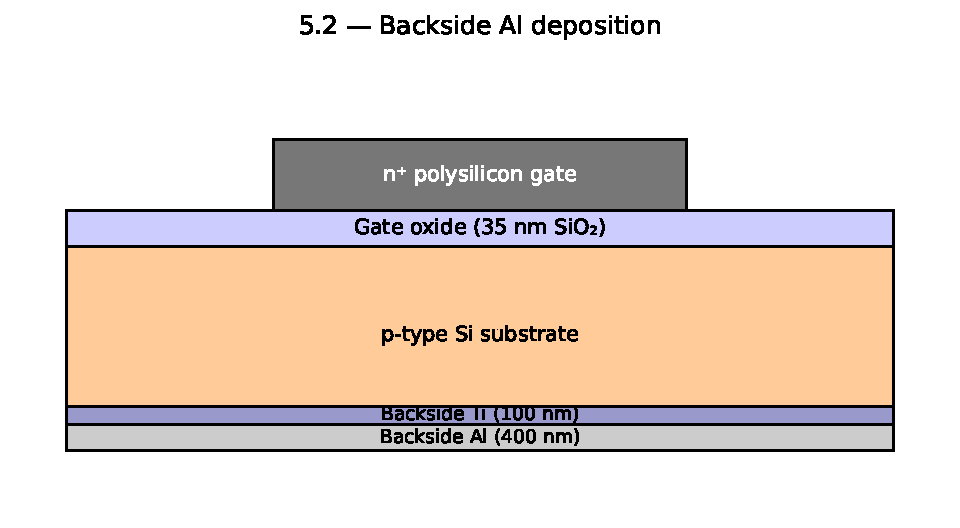
\includegraphics{figures/process_steps/moscap/moscap_step_5-2.pdf}}\\[2pt]
    Backside Al deposition
\end{minipage} \\

9 & 5.3 &
\begin{minipage}{\linewidth}
    \centering
    \resizebox{!}{3.5cm}{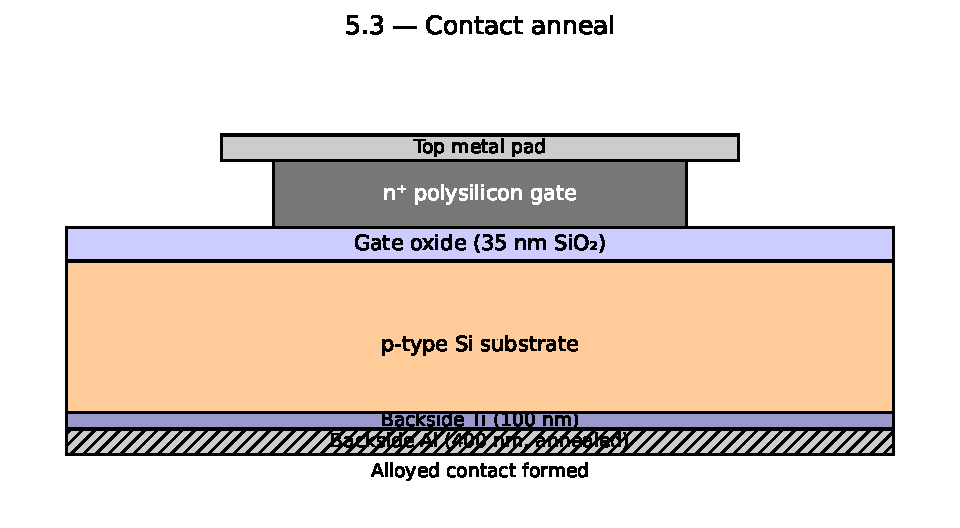
\includegraphics{figures/process_steps/moscap/moscap_step_5-3.pdf}}\\[2pt]
    Contact anneal
\end{minipage} \\

\end{longtblr}


\end{document}